Our primary objective is separating experimental data into two possible categories.
We hypothesize that the categories are linearly separable.
\section{Classification}

\subsection{Simulated data}
The simulated data contains two classes of events - single and double. 

\begin{table}
\centering
\caption{
Mean F1-scores and confusion matrix values for classification of simulated data 
using multiple models. Error estimates are the standard deviation in results from k-fold
cross-validation with $K=5$ folds.
}
\label{tab:classification-simulated}
\begin{tabular}{llllll}
\toprule
{} &                                            F1-score &                                                     TN &                                                     FP &                                                     FN &                                                     TP \\
\midrule
Logistic         &  $\underset{\num{+- 7.727e-03 }  }{\num{ 0.734 } }$ &  $\underset{\num{+- 1.546e+04 }  }{\num{ 1.28e+05 } }$ &  $\underset{\num{+- 1.546e+04 }  }{\num{ 6.16e+04 } }$ &  $\underset{\num{+- 1.118e+04 }  }{\num{ 4.39e+04 } }$ &  $\underset{\num{+- 1.118e+04 }  }{\num{ 1.46e+05 } }$ \\
Dense            &  $\underset{\num{+- 1.329e-02 }  }{\num{ 0.907 } }$ &  $\underset{\num{+- 1.125e+04 }  }{\num{ 1.72e+05 } }$ &  $\underset{\num{+- 1.125e+04 }  }{\num{ 1.85e+04 } }$ &  $\underset{\num{+- 5.205e+03 }  }{\num{ 1.73e+04 } }$ &  $\underset{\num{+- 5.205e+03 }  }{\num{ 1.73e+05 } }$ \\
Convolutional    &  $\underset{\num{+- 6.286e-03 }  }{\num{ 0.959 } }$ &  $\underset{\num{+- 7.287e+02 }  }{\num{ 1.89e+05 } }$ &  $\underset{\num{+- 7.290e+02 }  }{\num{ 1.39e+03 } }$ &  $\underset{\num{+- 2.692e+03 }  }{\num{ 1.37e+04 } }$ &  $\underset{\num{+- 2.692e+03 }  }{\num{ 1.76e+05 } }$ \\
Pretrained VGG16 &  $\underset{\num{+- 1.591e-02 }  }{\num{ 0.894 } }$ &  $\underset{\num{+- 9.079e+03 }  }{\num{ 1.79e+05 } }$ &  $\underset{\num{+- 9.080e+03 }  }{\num{ 1.15e+04 } }$ &  $\underset{\num{+- 9.409e+03 }  }{\num{ 2.71e+04 } }$ &  $\underset{\num{+- 9.408e+03 }  }{\num{ 1.63e+05 } }$ \\
\bottomrule
\end{tabular}
\end{table}

Classification results using models within a range of complexities are presented in table
\ref{tab:classification-simulated}.

\begin{figure}
\centering
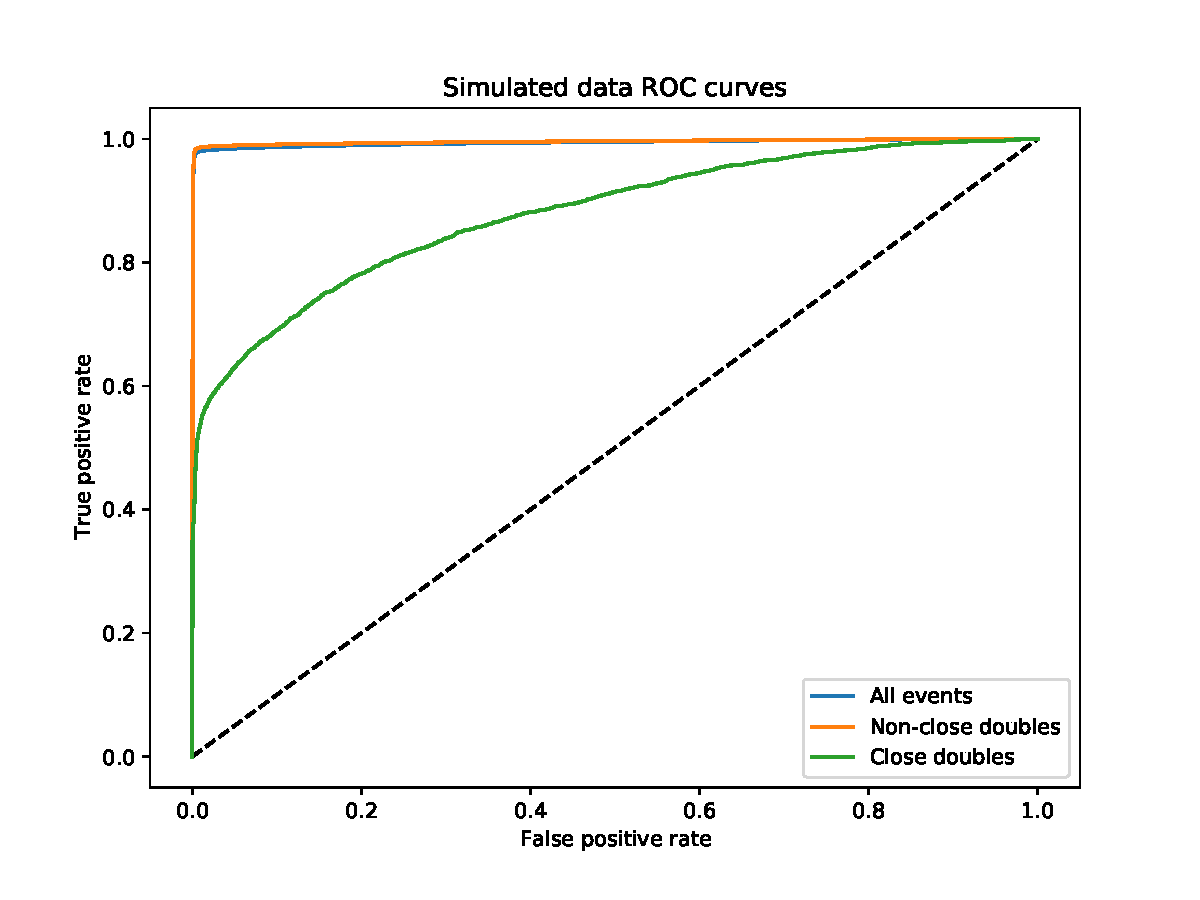
\includegraphics[width=0.8 \textwidth]{chapters/results/figures/roc_simulated.pdf}
\caption[Titletext]{generic text}\label{fig:roc_simulated}
\end{figure}

\subsection{Regression}
Same approach as for classification.
\begin{itemize}
  \item ? - Linear approach?
  \item ? - Dense network
  \item ? - CNN
\end{itemize}
\subsection{Experimental data}
\section{Regression}
\subsection{Position}
\subsection{Energy}
\subsection{Position}
\subsection{Energy}
